\documentclass{article}
\usepackage{graphicx}
\usepackage[margin=1.5cm]{geometry}
\usepackage{amsmath}

\begin{document}
\twocolumn

\title{Friday warm-up: Forces II}
\author{Prof. Jordan C. Hanson}

\maketitle

\section{Memory Bank}

\begin{itemize}
\item $\vec{r} = r\cos(\omega t)\hat{i} + r\sin(\omega t)\hat{j}$ ... Position for uniform circular motion, with angular velocity $\omega$.
\item $\vec{F}_{\rm C} = -m\vec{r}\omega^2$ ... The centripetal acceleration given the speed $v$ around a circular path $r$.
\item $\vec{f} = -\mu N \hat{i}$ ... Force of friction in the horizontal direction, given a normal force $N$.
\end{itemize}

\section{Forces, II}

\begin{enumerate}
\item Consider the banking plane in Fig. \ref{fig:1}.  Suppose the mass of the plane is $10^4$ kg.  (a) If the lift force $\vec{L}$ has a magnitude of $1.02 \times 10^5$ N, what is the bank angle such that the plane flies level? (b) What is the centripetal force? (c) Note that the \textit{period} $T$ of circular motion is $T = 2\pi/\omega$.  If $T$ for the motion of the plane is 2 minutes, what is the radius $r$ of the path? \\ \vspace{4cm}
\item Consider the parallel springs in Fig. \ref{fig:2}.  (a) If $k_1 = 15$ N m$^{-1}$, and $k_2 = 30$ N m$^{-1}$, what applied force will squeeze the springs by 5cm? (b) If instead the springs were connected \textit{in series} (back to back), convince yourself that 
\begin{equation}
k_1 \Delta x_1 = k_2 \Delta x_2 = k_{\rm total} \Delta x_{\rm total}
\end{equation}
Since $\Delta x_{\rm total} = \Delta x_1 + \Delta x_2$, solve for $k_{\rm total}$.  What is the equivalent formula for $k_{\rm total}$ for the parallel springs? \\ \vspace{4cm}
\item The force of friction is proportional to the normal force balancing the weight of a system. (a) Suppose the coefficient of kinetic friction $mu$ between rubber and concrete is 0.7, and 0.35 if the pavement is wet.  If the friction of sliding tires across pavement slows a vehicle from initial speed $v_i$ to a final speed $v_f = 0$, what is the ratio of stopping distances?  Assume the mass of the vehicle is $m$. (b) What is the stopping distance of a 2000 kg minivan on wet pavement, if $v_i = 100$ km per hour?
\end{enumerate}

\begin{figure}
\centering
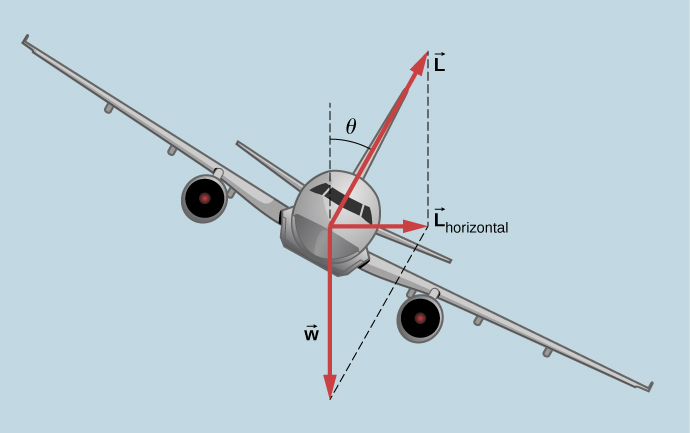
\includegraphics[width=0.4\textwidth]{figures/plane.jpeg}
\caption{\label{fig:1} A plane banks during flight, with the forces of lift and weight resulting in a centripetal force.}
\end{figure}

\begin{figure}
\centering
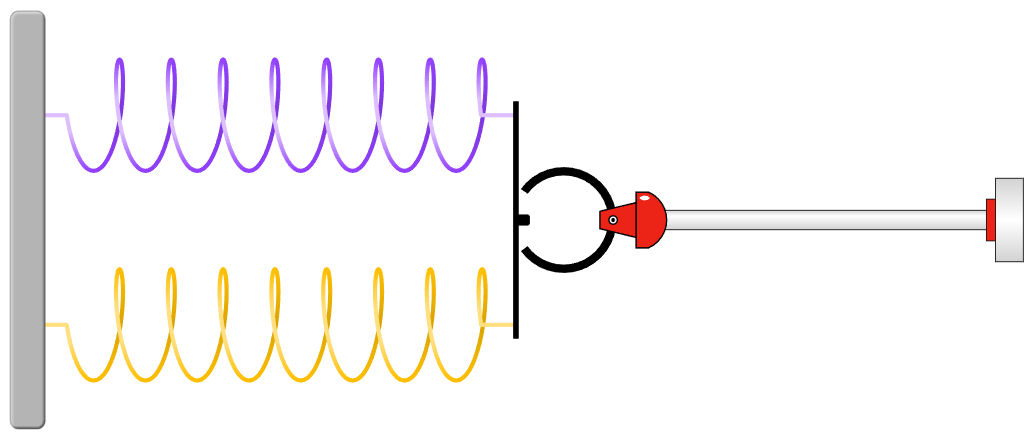
\includegraphics[width=0.33\textwidth]{figures/parallel_springs.png}
\caption{\label{fig:2} Two springs with $k_1$ and $k_2$, connected in parallel.}
\end{figure}

\end{document}
